% -------------------------------------------------------------------------------- %
% Latex file: `cropped-image.tex`
% Description:
% Speaking about cropped image cameramen details
% -------------------------------------------------------------------------------- %


% -------------------------------------------------------------------------------- %
\begin{frame}
    \frametitle{Selected Deep Nets Compression Techniques}
        % \centering \Huge
        \begin{center}
            {\fontsize{40}{50}\selectfont \emph{Input Dataset}}
        \end{center}
        \begin{center}
            \emph{Describing selected Input Target Image for our trials}
        \end{center}
        \begin{figure}
            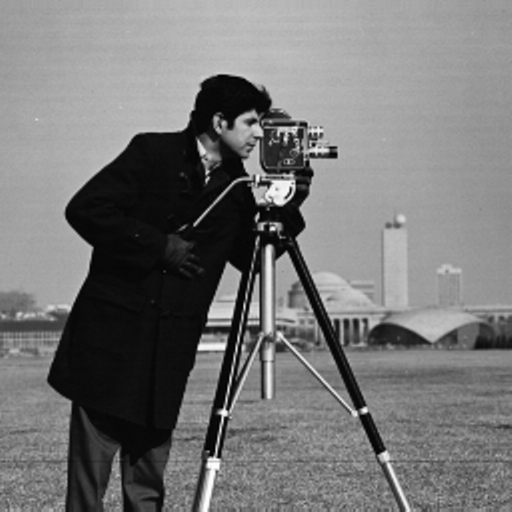
\includegraphics[scale=0.2]{slides/experiments/target-image/images/cameramen_512x512.png}
            \caption{Camera 512x512 cameramen image}
        \end{figure}
\end{frame}

% Target Image for Training Siren Models
% -------------------------------------------------------------------------------- %
\begin{frame}
    \frametitle{Target Image for Training Siren Models}
        Differently from Siren paper's Camera Image, we decide to resize it, by cropping the full image down to 256x256 image about its center,
        leading to the following update image:
        \begin{columns}
            \column{0.5\textwidth}
            \begin{figure}
            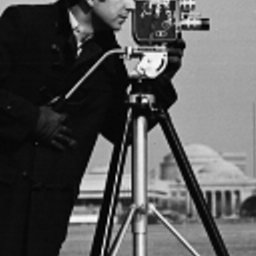
\includegraphics[scale=0.2]{slides/experiments/target-image/images/cropped_cameramen_256x256.png}
            \caption{Camera 256x256 target image}
            \end{figure}

        \column{0.5\textwidth}
            \begin{table}
                \begin{tabular}{ll}
                \hline
                        Image Feature & Value \\
                \hline
                    name &      Camera \\
                    shape &  (256, 256) \\
                size\_byte &       65536 \\
                image\_band &        (L,) \\
                \hline
                \end{tabular}
                \caption{Cropped Camera Image Characteristics }
            \end{table}
        \end{columns}
\end{frame}

% Data Distribution for Target Image for Training Siren Models
% -------------------------------------------------------------------------------- %
\begin{frame}
    \frametitle{Data Distribution for Target Image for Training Siren Models}
        \begin{figure}
        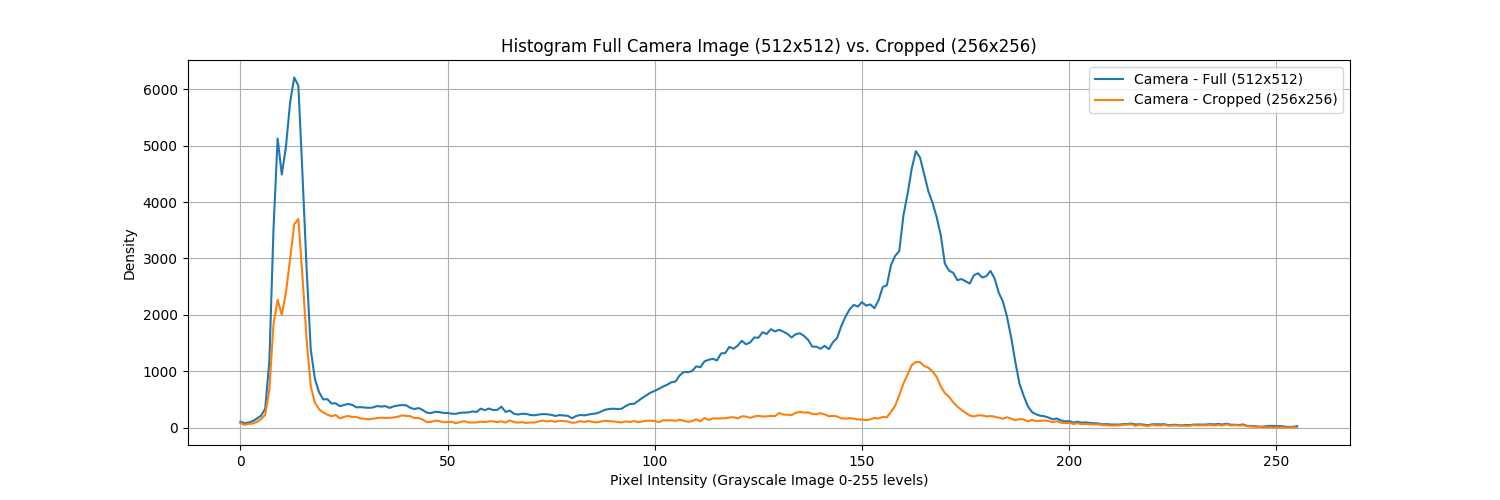
\includegraphics[scale=0.2]{slides/experiments/target-image/images/mixing_image_hist.png}
        \caption{Camera target image, full and cropped data distribution}
        \end{figure}
\end{frame}


% General Summarizing Image Overview
% -------------------------------------------------------------------------------- %
\begin{frame}
    \frametitle{General Summarizing Image Overview}
        \begin{figure}
        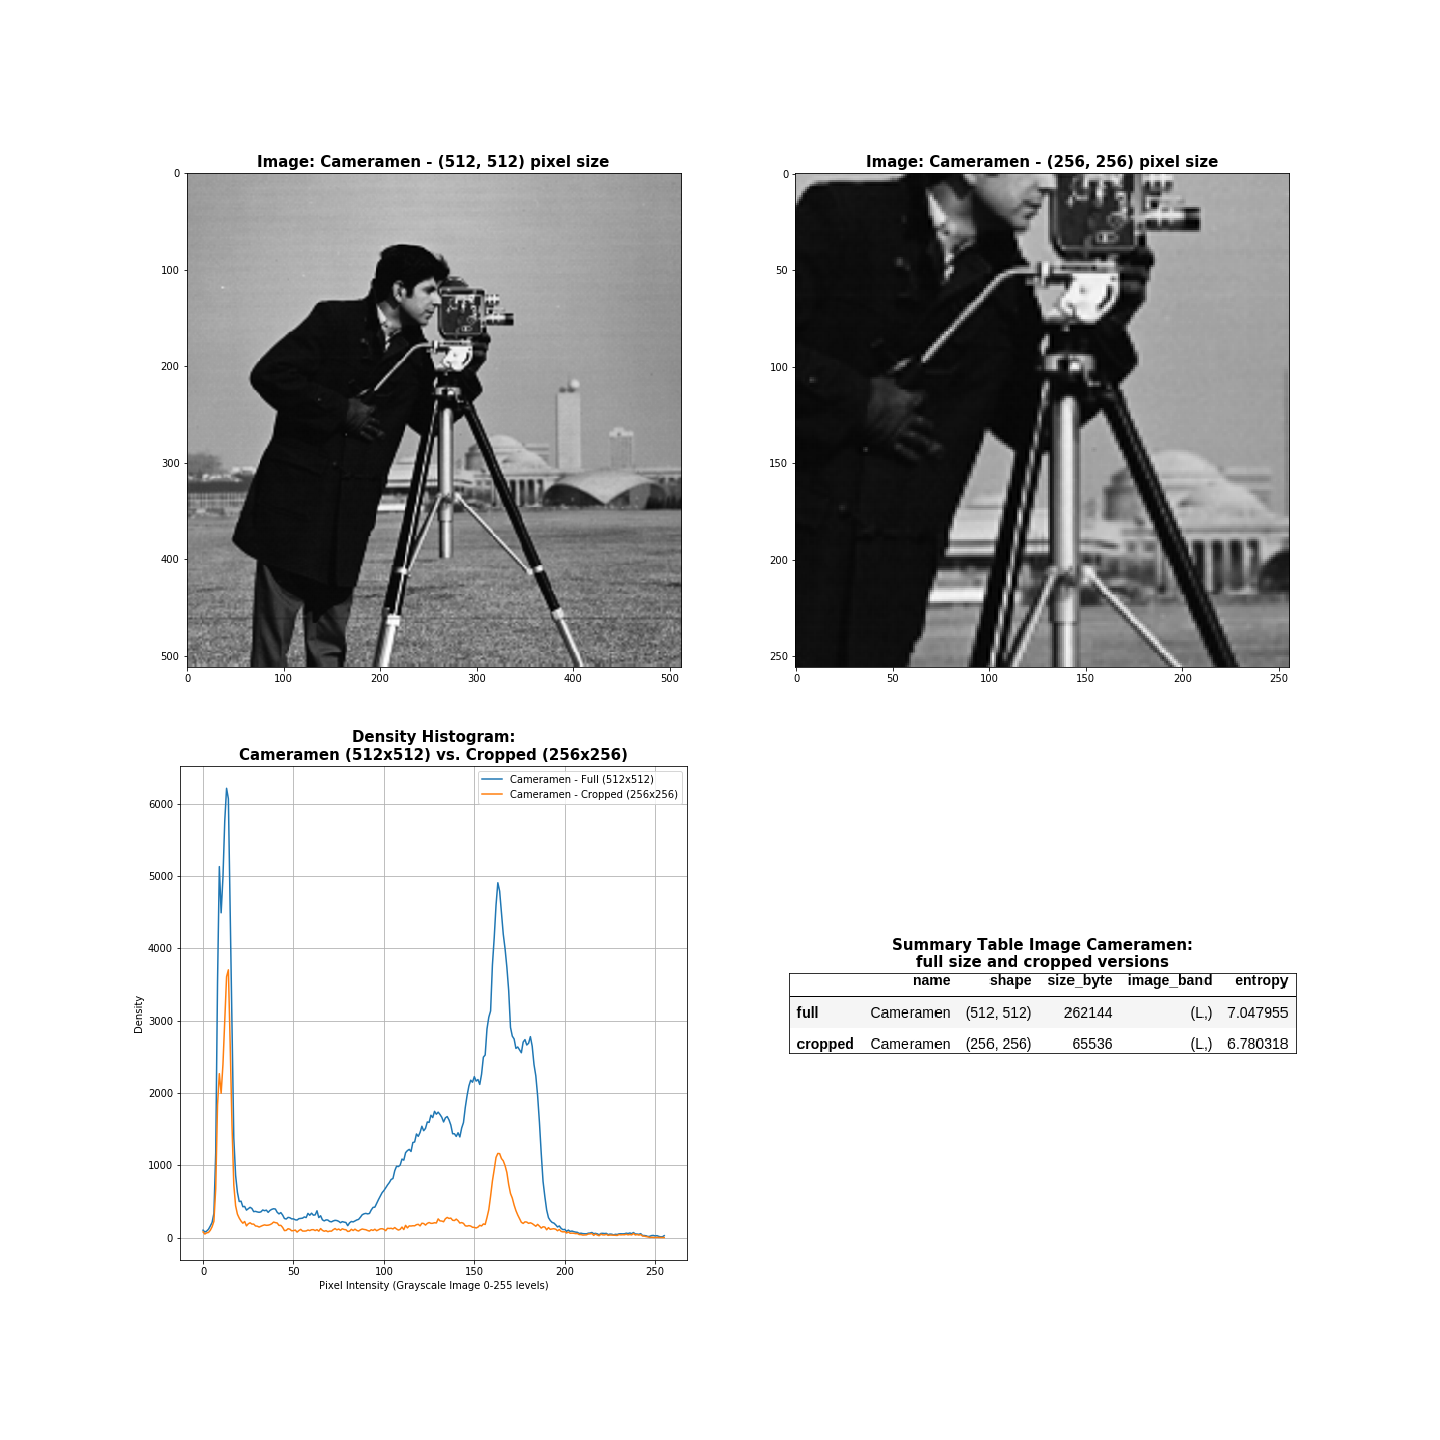
\includegraphics[scale=0.15]{slides/experiments/target-image/images/complex_3.png}
        \end{figure}
\end{frame}
